	% 代码分析:模块功能、涉及到的类、类关系、数据结构及关键代码等;
	% 任务要求,设计任务要求;
	% 设计:详细的设计方案,相关的数据结构、算法描述,可采用伪代码等形式化描述
	% 实现:修改哪些类、如何修改、为什么修改等;
	% 测试:测试用例,测试结果及结果分析,测试运行界面等;
	% 调试:调试方法,遇到的问题及解决方案等;
	% 结论与展望:完成的主要工作、收获、进一步的工作,建议、体会、心得等;

\section{作业3}
\subsection{作业3.1}
\subsubsection{题目描述}

C 风格变量声明的正规式:

\[(i|r)v(,v)^*;\]

其中 $i$ 和 $r$ 分别表示整型和实型数据类型,$v$ 表示变量名。

\begin{enumerate}
    \item 构造NFA,并单符化。
    \item 确定化。
    \item 最小化。
\end{enumerate}

\subsubsection{解答}

\paragraph{构造NFA,并单符化。} 按照给出的步骤,不难画出:

\begin{figure}[H]
    \centering
    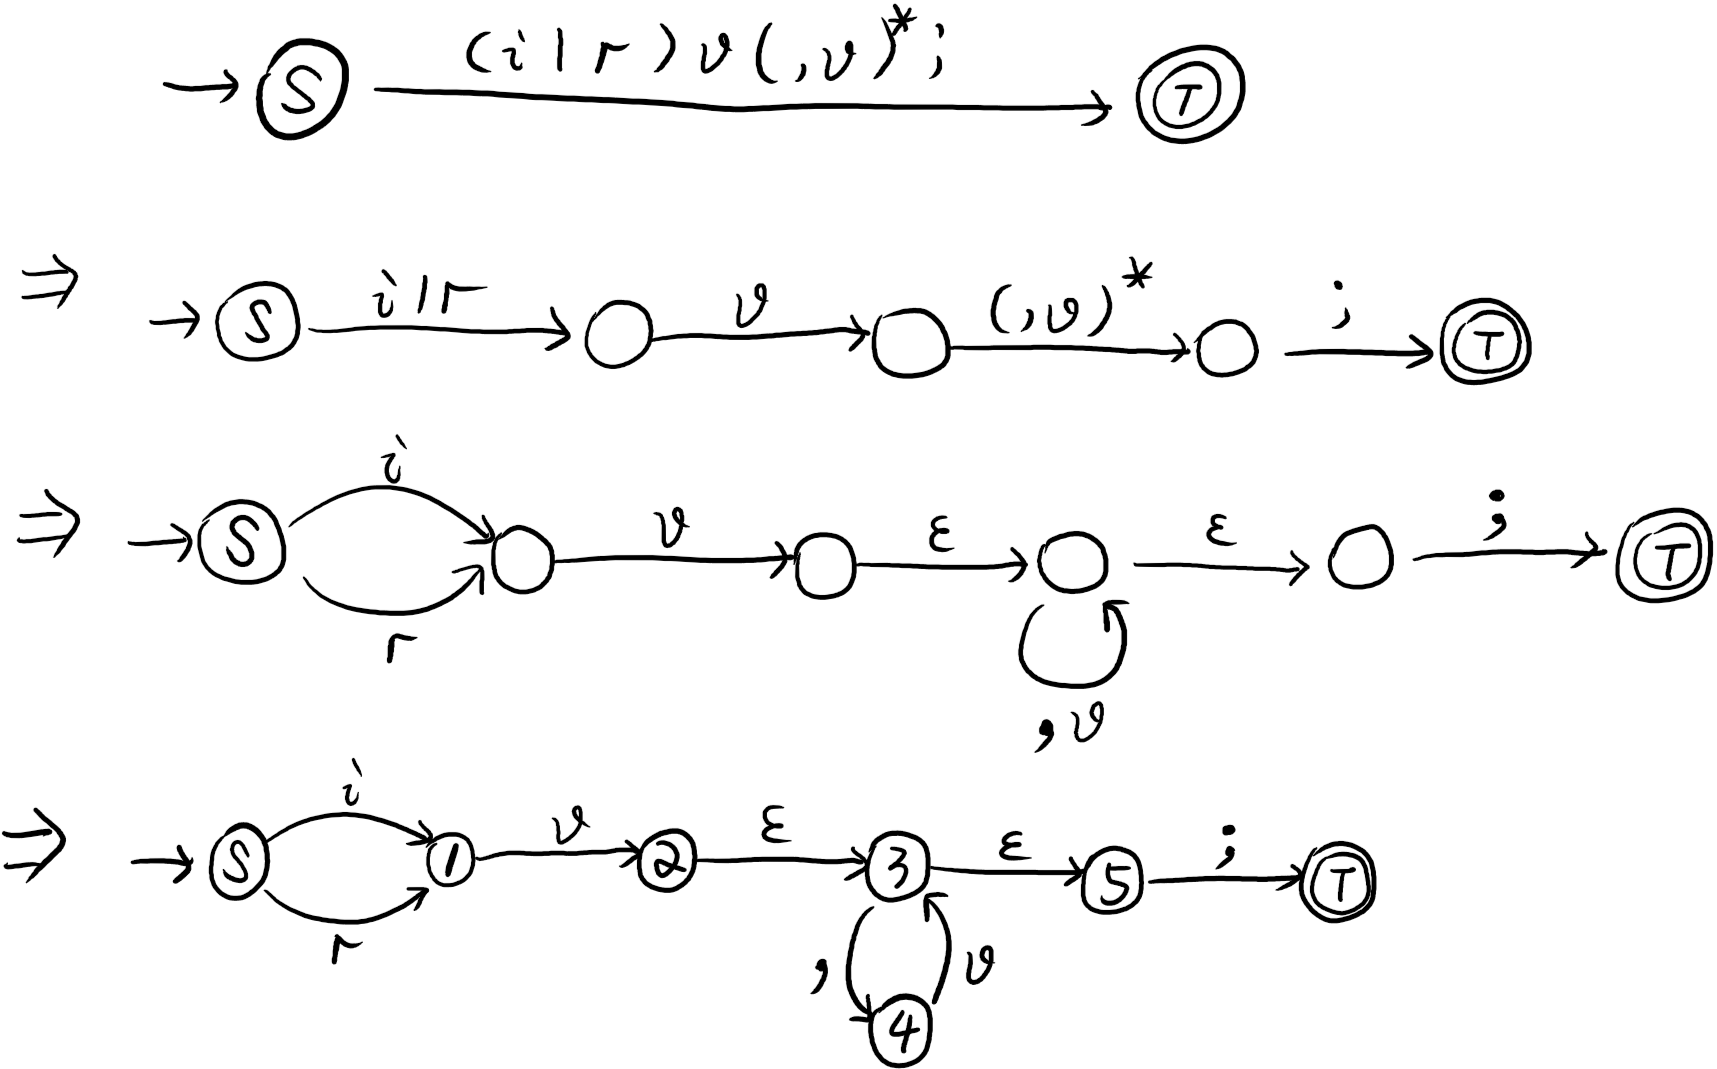
\includegraphics[width=0.8\linewidth]{imgs/3.png}
    \caption{正则 $r$ $\Rightarrow\;$NFA $M$}
    \label{fig:NFA}
\end{figure}

\paragraph{确定化。} 对于上面画出的NFA,首先设字母表为 $\Sigma=\left\{i,r,',',v,';'\right\}$,初态为 $X$,可以写出闭包:

\begin{center}
\begin{tikzpicture}[>=stealth',shorten >=1pt,auto,node distance=2cm]
  \node[initial,state] (X)      {$X$};
  \node[state]         (q1) [right of=X]  {$q_1$};
  \node[state]         (q2) [right of=q1] {$q_2$};
  \node[state]         (q3) [right of=q2] {$q_3$};
  \node[state]         (q4) [below of=q3] {$q_4$};
  \node[state]         (q5) [right of=q3] {$q_5$};
  \node[state,accepting](Y) [right of=q5] {$Y$};

  \path[->]  (X)  edge[bend right] node {$r$} (q1);
  \path[->]  (X)  edge[bend left] node {$i$} (q1);
  \path[->]  (q1)  edge node {$v$} (q2);
  \path[->]  (q2)  edge node {$\varepsilon$} (q3);
  \path[->]  (q3)  edge node {$\varepsilon$} (q5);
  \path[->]  (q5)  edge node {$;$} (Y);
  \path[->]  (q3)  edge[bend left] node {$,$} (q4);
  \path[->]  (q4)  edge[bend left] node {$v$} (q3);
\end{tikzpicture}
\end{center}


\begin{table}[H]
    \centering
    \begin{tabular}{>{\bfseries}c *5{c}}
        \toprule
        $I$ & $I_r$ & $I_i$ & $I_v$ & $I_,$ & $I_;$\\
        \midrule
        $\{X\}$ & $\{q_1\}$ & $\{q_1\}$ & $\Phi$ & $\Phi$ & $\Phi$\\
        $\{q_1\}$ & $\Phi$ & $\Phi$ & $\{q_2, q_3, q_5\}$ & $\Phi$ & $\Phi$\\
        $\{q_2, q_3, q_5\}$ & $\Phi$ & $\Phi$ & $\Phi$ & $\{q_4\}$ & $\{Y\}$\\
        $\{q_4\}$ & $\Phi$ & $\Phi$ & $\{q_3, q_5\}$ & $\Phi$ & $\Phi$\\
        $\{q_3, q_5\}$ & $\Phi$ & $\Phi$ & $\Phi$ & $\{q_4\}$ & $\{Y\}$\\
        $\{Y\}$ & $\Phi$ & $\Phi$ & $\Phi$ & $\Phi$ & $\Phi$\\
        \bottomrule
    \end{tabular}
    \caption{$\delta^\prime:\; S\times\Sigma\to S$}
    \label{tab:my_label}
\end{table}

可以按次序编号为:

\begin{table}[H]
    \centering
    \begin{tabular}{>{\bfseries}c *5{c}}
        \toprule
        $I$ & $I_r$ & $I_i$ & $I_v$ & $I_,$ & $I_;$\\
        \midrule
        $S$ & $1$ & $1$ &  &  & \\
        $1$ &  &  & $2$ &  & \\
        $2$ &  &  &  & $3$ & $T$\\
        $3$ &  &  & $4$ &  & \\
        $4$ &  &  &  & $3$ & $T$\\
        $T$ &  &  &  &  & \\
        \bottomrule
    \end{tabular}
    \caption{$\delta^\prime:\; S\times\Sigma\to S$}
    \label{tab:my_label}
\end{table}

根据 $\delta^\prime$ 可以画出:

\begin{center}
\begin{tikzpicture}[>=stealth',shorten >=1pt,auto,node distance=2cm]
  \node[initial,state] (X)      {$S$};
  \node[state]         (q1) [right of=X]  {$1$};
  \node[state]         (q235) [right of=q1] {$2$};
  \node[state]         (q4) [below of=q235] {$3$};
  \node[state]         (q35) [right of=q4] {$4$};
  \node[state,accepting](Y) [right of=q235] {$T$};

  \path[->]  (X)  edge[bend right] node {$r$} (q1);
  \path[->]  (X)  edge[bend left] node {$i$} (q1);
  \path[->]  (q1)  edge node {$v$} (q235);
  \path[->]  (q235)  edge node {$;$} (Y);
  \path[->]  (q235)  edge node {$,$} (q4);
  \path[<-]  (q4)  edge[bend right] node {$,$} (q35);
  \path[->]  (q4)  edge[bend left] node {$v$} (q35);
  \path[->]  (q35)  edge node {$;$} (Y);
\end{tikzpicture}
\end{center}

\paragraph{最小化。} 在上表中可以看出 2 与 4 对应的列完全相同,故其为等价状态,可以合并为:

\begin{center}
\begin{tikzpicture}[>=stealth',shorten >=1pt,auto,node distance=2cm]
  \node[initial,state] (X)      {$S$};
  \node[state]         (q1) [right of=X]  {$1$};
  \node[state]         (q235) [right of=q1] {$2,4$};
  \node[state]         (q4) [below of=q235] {$3$};
  \node[state,accepting](Y) [right of=q235] {$T$};

  \path[->]  (X)  edge[bend right] node {$r$} (q1);
  \path[->]  (X)  edge[bend left] node {$i$} (q1);
  \path[->]  (q1)  edge node {$v$} (q235);
  \path[->]  (q235)  edge node {$;$} (Y);
  \path[->]  (q235)  edge[bend left] node {$,$} (q4);
  \path[->]  (q4)  edge[bend left] node {$v$} (q235);
\end{tikzpicture}
\end{center}

此时将 $2,4$ 编号为 $2^\prime$,编号表格为:

\begin{table}[H]
    \centering
    \begin{tabular}{>{\bfseries}c *5{c}}
        \toprule
        $I$ & $I_r$ & $I_i$ & $I_v$ & $I_,$ & $I_;$\\
        \midrule
        $S$ & $1$ & $1$ &  &  & \\
        $1$ &  &  & $2^\prime$ &  & \\
        $2^\prime$ &  &  &  & $3$ & $T$\\
        $3$ &  &  & $2^\prime$ &  & \\
        $T$ &  &  &  &  & \\
        \bottomrule
    \end{tabular}
    \caption{$\delta^\prime:\; S\times\Sigma\to S$}
    \label{tab:my_label}
\end{table}

可以看到 $1$ 与 $3$ 完全相同,记为 $1^\prime$,可以化简为:

\begin{center}
\begin{tikzpicture}[>=stealth',shorten >=1pt,auto,node distance=2cm]
  \node[initial,state] (X)      {$S$};
  \node[state]         (q1) [right of=X]  {$1^\prime$};
  \node[state]         (q235) [right of=q1] {$2^\prime$};
  \node[state,accepting](Y) [right of=q235] {$T$};

  \path[->]  (X)  edge[bend right] node {$r$} (q1);
  \path[->]  (X)  edge[bend left] node {$i$} (q1);
  \path[->]  (q1)  edge[bend left] node {$v$} (q235);
  \path[<-]  (q1)  edge[bend right] node {$,$} (q235);
  \path[->]  (q235)  edge node {$;$} (Y);
\end{tikzpicture}
\end{center}

此时编号表格为:

\begin{table}[H]
    \centering
    \begin{tabular}{>{\bfseries}c *5{c}}
        \toprule
        $I$ & $I_r$ & $I_i$ & $I_v$ & $I_,$ & $I_;$\\
        \midrule
        $S$ & $1$ & $1$ &  &  & \\
        $1^\prime$ &  &  & $2^\prime$ &  & \\
        $2^\prime$ &  &  &  & $3$ & $T$\\
        $T$ &  &  &  &  & \\
        \bottomrule
    \end{tabular}
    \caption{$\delta^\prime:\; S\times\Sigma\to S$}
    \label{tab:my_label}
\end{table}


每列有且仅有一种转移,是最小化的充分条件,故此时为最小化 DFA。

% \subsection{作业1.2}
% \subsubsection{题目描述}
% \subsubsection{解答}

% \subsection{作业1.3}
% \subsubsection{题目描述}
% \subsubsection{解答}